% A Clock in the Loop: Request-Time Temporal Grounding for Long-Context Agent Workflows
%
% DRAFT — compile with: pdflatex paper.tex
% For ICLR submission, swap the preamble for the official ICLR style files
% (iclr2027.sty / iclr2026.sty) and anonymize author fields.
\documentclass[10pt]{article}

\usepackage[margin=1in]{geometry}
\usepackage{amsmath,amssymb}
\usepackage{booktabs}
\usepackage{graphicx}
\usepackage{xcolor}
\usepackage{enumitem}
\usepackage{titlesec}
\usepackage{caption}
\captionsetup{font=small,labelfont=bf}
\titlespacing*{\section}{0pt}{1.1em}{0.45em}
\titlespacing*{\subsection}{0pt}{0.8em}{0.3em}
\setlength{\parskip}{0.15em}

\definecolor{seablue}{RGB}{29,95,158}
\definecolor{seaaccent}{RGB}{56,182,216}
\usepackage[colorlinks=true,linkcolor=seablue,urlcolor=seablue,citecolor=seablue]{hyperref}

\title{\bfseries A Clock in the Loop:\\[1pt] Request-Time Temporal Grounding for Long-Context Agent Workflows}
\author{Anonymous submission\\[2pt] (arXiv version: DeepSeek Code project)}
\date{\today}

\begin{document}
\maketitle

\begin{abstract}
Autonomous LLM agents operate in long-lived sessions in which tool results, reasoning
traces, and user messages accumulate inside a single context window. Because LLMs
cannot perceive wall-clock time, stale observations are routinely treated as current:
yesterday's test output is cited as today's state, and still-fresh data is needlessly
re-fetched. The problem is amplified by 1M-token context windows, where outdated
content can survive for days. We present the \emph{Time Awareness Layer} (TAL), a
request-time temporal grounding mechanism for agent harnesses, implemented in
DeepSeek Code, a desktop IDE built around DeepSeek's 1M-token models. TAL injects a
live clock, per-message timestamps with bucketed ages, per-tool freshness horizons
stamped onto tool results, and conversation-span notes for long sessions---without
modifying stored history, while preserving Anthropic-protocol tool-result adjacency,
and while keeping prefix-cache invalidation confined to the tail of the input. We
evaluate TAL on DeepSeek V4 Flash and V4 Pro with a three-probe benchmark (72
tool-alignment cases, 72 audit claims, and 9 duration tasks per model). TAL raises
T1 tool-call alignment from 62.5\% to 91.7\% (Flash) and from 44.4\% to 100\%
(Pro), with non-overlapping 95\% Wilson intervals. An adversarial label-flip
control, however, collapses T1 accuracy to 26--31\%, showing that the model largely
\emph{follows} the explicit freshness label. A one-line decision procedure
(``compute the age, compare it against the horizon, and treat the label as
potentially wrong'') recovers 98.6\% accuracy under the same adversarially flipped
labels in both models --- evidence that the gap is reasoning depth, not model
capability, and that temporal grounding should pair stamps with an explicit
decision procedure. T3 gains are modest (+2.8 points, concentrated in ordering
violations), and T2 reveals that Flash overestimates its own runtime (median
3.7$\times$) while Pro underestimates it (median 0.56$\times$). A cache probe shows
TAL preserves DeepSeek prefix-cache hits (99.5\% vs.\ 98.0\% cached share) at a cost
of roughly 22 tokens per message. The implementation and benchmark are released with
the paper.
\end{abstract}

\section{Introduction}
\label{sec:intro}

Agentic LLM workflows are conversations with a filesystem: the model reads files,
runs commands, searches the web, and edits code, with every observation appended to a
context window that may live for hours or days. This design has a hidden cost. A
model has no intrinsic sense of elapsed time; it only knows what the text says. When
an observation from yesterday sits next to an observation from two minutes ago, the
model has no reliable way to tell them apart, so it often treats both as describing
the present. Recent work confirms the problem is structural: LLMs misestimate their
own runtime by 4--7$\times$ \cite{perceive_time}, and multi-turn models silently
drift from an established temporal scope back to the present \cite{chronoscope}.

Long-context systems make this worse in a specific way. A 1M-token window does not
just \emph{allow} long sessions; it \emph{encourages} them, and it changes what
``stale'' means. In a short session, an old tool result is likely to be compacted
away or forgotten. In a million-token session, an 80k-token file listing from three
days ago sits fully visible, verbatim, indistinguishable in presentation from a
result fetched ten seconds ago. The very feature that makes long context powerful
--- retaining everything --- becomes the mechanism by which temporal error persists.

Our position is that agent harnesses should make time \emph{legible} to the model at
the moment it matters: at request time, when the model decides whether to trust,
reuse, re-fetch, or flag an observation. We make three contributions:

\begin{enumerate}[leftmargin=1.4em,itemsep=1pt]
  \item \textbf{Design.} We specify a lightweight Time Awareness Layer (TAL) with four
        injection points --- a live clock, per-message age stamps, per-tool freshness
        horizons on tool results, and conversation-span notes --- and articulate two
        design principles that make it practical in production: \emph{derive, don't
        store} (stamps are applied at request time so stored history stays clean and
        ages never go stale), and \emph{cache-conscious placement} (bucketed ages and
        an end-of-input clock confine prefix-cache invalidation to the final message).
  \item \textbf{Implementation.} We integrate TAL into DeepSeek Code, a Tauri-based
        IDE built around DeepSeek V4's 1M-token context, including protocol-safe
        stamping of tool results and high-fidelity session restore that survives
        model switches and restarts.
  \item \textbf{Evaluation.} We build a scalable three-probe benchmark with an
        ablation protocol and run it on DeepSeek V4 Flash and V4 Pro (72 cases per
        condition). T1 tool-call alignment improves by +29.2 (Flash) and +55.6
        (Pro) points; an adversarial label-flip control drops accuracy to
        26--31\%, exposing label-following; and a decision-chain prompt recovers
        98.6\% under flipped labels in both models, closing the age-reasoning gap.
        T3 gains are modest and concentrated in ordering violations; the two models
        miscalibrate their own runtime in opposite directions; and a cache probe
        quantifies the cost of temporal stamping at roughly 22 tokens per message.
\end{enumerate}

\section{Background and Related Work}
\label{sec:related}

\textbf{Temporal reasoning benchmarks.} \emph{Test of Time} \cite{testoftime}
introduced synthetic datasets probing temporal reasoning across orderings,
arithmetic, and consistency, and found current LLMs far below human performance.
\emph{MegaTempQA} \cite{megatempqa} scales temporal QA to a million pairs and uses it
as a diagnostic for temporal hallucination. \emph{ChronoScope} \cite{chronoscope}
constructs over a million controlled multi-turn chains to isolate \emph{temporal
drift} --- the bias toward the present when follow-ups omit time references --- and
proposes chain-consistency metrics. These benchmarks measure static reasoning; our
work instead measures a \emph{harness intervention} on an operating agent loop.

\textbf{Time perception.} \emph{Can LLMs Perceive Time?} \cite{perceive_time}
experiments across 68 tasks and four model families show that LLMs overestimate their
own task duration by roughly 4--7$\times$, cannot order durations reliably, and remain
miscalibrated even after finishing. \emph{Discrete Minds in a Continuous World}
\cite{token_time} proposes a Token-Time Hypothesis: models connect text length to
elapsed time but have no direct clock signal. Our T2 probe reproduces the
overestimation pattern on DeepSeek V4 Flash (median 3.71$\times$, $n{=}9$), while
DeepSeek V4 Pro \emph{underestimates} its runtime (median 0.56$\times$) ---
opposite directions within one family. TAL is explicitly designed to supply the
missing external clock signal that these works identify.

\textbf{Temporal validity in memory.} \emph{MemStrata} \cite{memstrata} maintains
temporal validity in retrieval memory by deterministically superseding contradicted
facts in a bi-temporal ledger, eliminating stale-fact errors for knowledge
retrieval. MemStrata operates at \emph{storage} time and targets fact-level updates;
TAL operates at \emph{request} time and targets observation-level staleness (tool
results, shell state, file reads). The two are complementary: storage-time
supersession keeps memory clean, request-time stamping keeps the model's \emph{use}
of memory temporally grounded.

\textbf{Context management in agent harnesses.} Production harnesses mitigate
unbounded growth with compression: Claude Code uses a multi-stage compaction
pipeline, and Codex exposes API-side \texttt{/responses/compact}. Compression trades
information for size; TAL trades a few hundred tokens for temporal precision and is
orthogonal to compression. Our system also differs from those harnesses in scale:
DeepSeek Code keeps the entire project in a 1M-token window by design
\cite{deepseek_context}, so temporal grounding is not a niche concern but a
first-order correctness issue.

\section{System: DeepSeek Code}
\label{sec:system}

DeepSeek Code is a desktop IDE (Tauri 2 + React) designed specifically for
DeepSeek's Anthropic-compatible endpoint. Its distinguishing features are relevant
here because they set the constraints under which TAL must operate:

\begin{itemize}[leftmargin=1.4em,itemsep=1pt]
  \item \textbf{1M-token, no-compression-first context.} The context engine indexes
        the project tree and key files at session start and only triggers ``soft
        forget'' above 900K tokens, preserving user messages and reasoning traces
        while trimming old tool outputs. This is what makes long sessions the common
        case and temporal error persistent.
  \item \textbf{Protocol-level parallelism.} Tool calls execute concurrently
        (capped at four) and merge into a single \texttt{tool\_result} message, as
        the Anthropic protocol requires. Every \texttt{tool\_use} id is registered
        before spawning so that even a failed task is answered with its real id.
  \item \textbf{Persistent sessions.} Conversations are saved to disk by the backend
        (backend-authoritative snapshots) and restored with full content blocks,
        supporting live model switches and restarts without context loss.
  \item \textbf{Prompt-cache accounting.} The agent tracks cached input tokens and
        USD savings from DeepSeek's prompt cache, making cache behavior a first-class
        design constraint rather than an afterthought.
\end{itemize}

\section{The Time Awareness Layer}
\label{sec:tal}

\subsection{Design: four injection points}
\label{sec:design}

We model temporal grounding as a stack of capabilities, and map each to an explicit,
measurable injection point in the harness:

\begin{description}[leftmargin=2.2em,itemsep=2pt]
  \item[L0 --- clock.] The model must know \emph{now}. TAL appends a live
        \texttt{[time\_harness now=...]} stamp to the last user message of every
        request. The stamp is re-derived per request, so it never goes stale even in
        a long-running turn loop.
  \item[L1 --- freshness.] The model must know how old each observation is and
        whether that age is acceptable for the claim at hand. Freshly produced tool
        results are stamped \texttt{[data\_time=... age=0min freshness=just\_fetched
        horizon=...]}; per-tool horizons (Section~\ref{sec:horizons}) let the model
        compare age against a decision threshold instead of guessing. Every message
        additionally receives \texttt{[message\_time=... age=...]}.
  \item[L2 --- proactive duration (measured, not yet closed).] The model must be able
        to estimate how long its own work will take so the harness can schedule
        operations and set expectations. Our T2 probe \emph{characterizes} the gap on
        DeepSeek V4 Flash; closing it (an L2 estimator + budget enforcement) is future
        work (Section~\ref{sec:future}).
  \item[L3/L4 --- temporal intentionality and narrative span.] The model must treat
        the conversation itself as having a temporal arc. For sessions spanning more
        than an hour, TAL prepends a span note to the first message:
        \emph{``this conversation spans from 2d ago... live data mentioned in older
        messages may be stale''}, and T3 measures the model's ability to audit logs
        for ordering and staleness violations.
\end{description}

\begin{figure}[t]
  \centering
  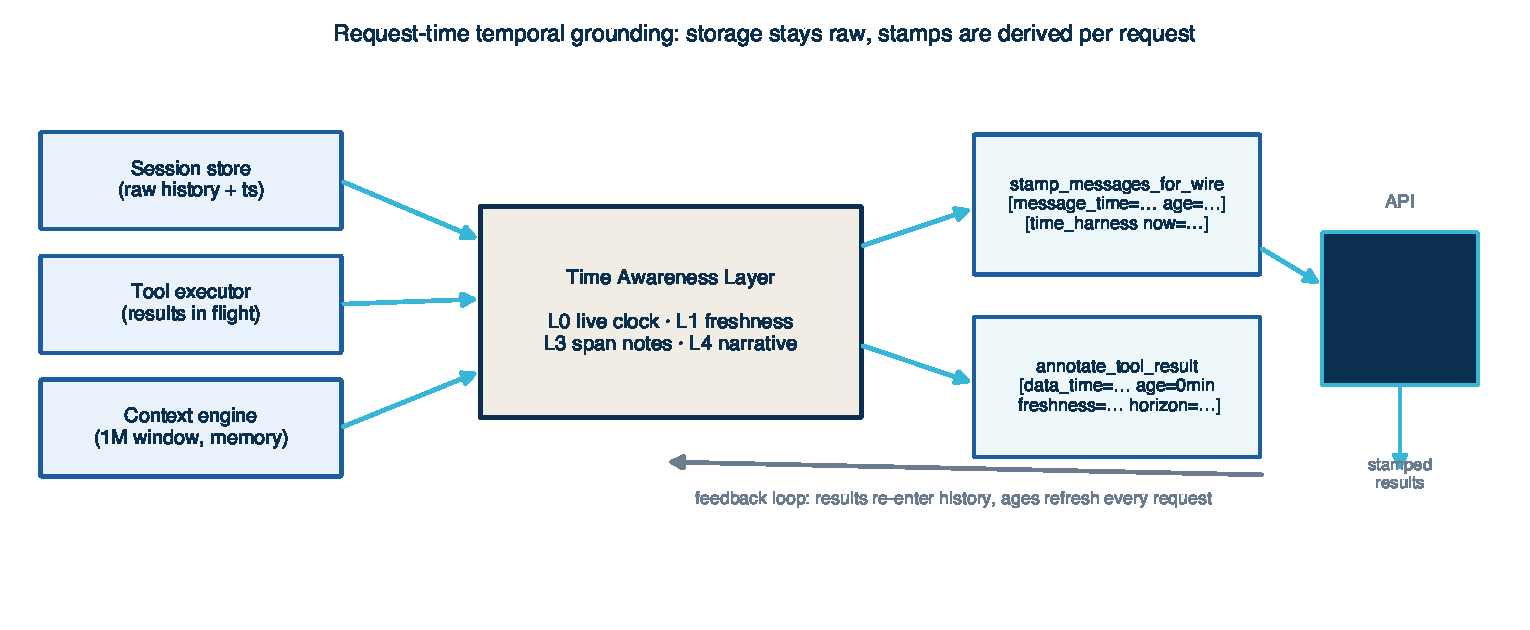
\includegraphics[width=0.98\linewidth]{figures/fig1_architecture.pdf}
  \caption{Request-time temporal grounding. Stored history and tool outputs stay
  raw; per-request stamps are derived at wire time, and stamped results re-enter
  history so ages refresh on the next request.}
  \label{fig:arch}
\end{figure}

\subsection{Design principles}
\label{sec:principles}

\textbf{Derive, don't store.} Stamps are applied to a clone of the message list at
request time (\texttt{stamp\_messages\_for\_wire}); stored sessions keep raw
content. This has three consequences: (i) history is never polluted by stamps, so
restoring a session can never double-stamp; (ii) ages are always computed against the
current clock, so a turn that lasts an hour still reports correct ages; (iii) the
harness is toggleable for ablation at runtime without migration.

\textbf{Cache-conscious placement.} DeepSeek prices prompt-cache reads below full
input, and cache hits require a byte-identical prefix. TAL keeps the prefix stable in
two ways. First, ages are bucketed (minutes, hours, days), so \texttt{age=2d} stays
byte-identical until the bucket rolls over; within a bucket the entire history prefix
is unchanged. Second, the live clock lives at the \emph{end} of the input (last user
message), so only the final segment changes between requests. The system prompt is
clock-free by construction: a clock embedded at session initialization would go
stale within the hour and create a second, conflicting time source (an IDE
self-audit caught exactly this conflict before the fix), while refreshing it per
turn would invalidate the entire prefix. The end-of-input stamp is therefore the
single authoritative clock.

\textbf{Protocol safety.} DeepSeek's Anthropic-compatible endpoint validates that
every \texttt{tool\_use} is immediately followed by its \texttt{tool\_result};
inserting a text stamp before a \texttt{tool\_result} block yields HTTP 400. TAL
therefore skips message-level stamps on tool-result messages --- their content blocks
already carry \texttt{[data\_time=...]} --- and only prepends text blocks to
plain-text and assistant messages.

\subsection{Freshness horizons}
\label{sec:horizons}

Freshness is claim-dependent: a stock quote and a file's contents do not expire on
the same schedule. TAL attaches a per-tool horizon at stamp time and mirrors the same
table in the system prompt:

\begin{table}[h]
  \centering
  \small
  \begin{tabular}{ll}
    \toprule
    Tool class & Freshness horizon \\
    \midrule
    stock / weather quotes & 15--30 min \\
    package tracking & 6 h \\
    web search & 24 h \\
    shell / system state & 1 h \\
    file contents & no expiry (re-read if the user asks about current state) \\
    \bottomrule
  \end{tabular}
  \caption{Per-tool freshness horizons exposed both in the stamp and in the system
  prompt, so the model compares age against a decision threshold directly.}
  \label{tab:horizons}
\end{table}

\subsection{Implementation notes}
\label{sec:impl}

The Rust harness implements the layer in three functions:
\begin{itemize}[leftmargin=1.4em,itemsep=1pt]
  \item \texttt{time\_harness\_system\_section(now)} --- the rules block appended to
        the system prompt, listing the freshness semantics and horizons.
  \item \texttt{annotate\_tool\_result(tool, content, now)} --- wraps every
        successful tool result with \verb![data_time=... age=0min freshness=just_fetched horizon=...]!.
  \item \texttt{stamp\_messages\_for\_wire(messages, now, enabled)} --- derives
        per-message stamps, the conversation span note, and the live end-of-input
        clock. The same code path serves both fresh turns and restored sessions.
\end{itemize}

Session persistence was upgraded in tandem. \texttt{StoredMessage} now carries
\texttt{blocks: Option<Vec<ContentBlock>>}, so saved conversations include full
tool-use/tool-result/web-search blocks rather than flattened text; the backend
snapshots messages authoritatively at save time, and \texttt{restore\_session}
rebuilds the exact message structure before TAL stamps it for the wire. This is what
makes ``yesterday's session, resumed today'' the canonical TAL scenario: restored
history gets correct, current ages, and the model sees the conversation span note,
instead of implicitly treating old content as fresh.

The system prompt deliberately contains no clock: refreshing \texttt{now} inside it
per turn would invalidate the entire prefix cache on every request, and freezing it
at session start would create a stale second clock source. The per-request
end-of-input stamp is the single authoritative time; server-side web-search results
are stamped on arrival (\texttt{horizon=24h}) alongside client tool results.

\section{Evaluation}
\label{sec:eval}

\subsection{Protocol}
\label{sec:protocol}

We measure the layer with three probes against DeepSeek V4 Flash and V4 Pro
(temperature 0, thinking disabled for probe stability) through the same
Anthropic-compatible endpoint the IDE uses. Each probe runs under two conditions:
\emph{baseline} (no harness annotations) and \emph{with TAL}. The benchmark harness
mirrors the production prompt and stamp formats exactly. Cases are generated
programmatically (two seeds, deterministic): 72 T1 cases, 24 T3 logs (72 claims),
and 9 T2 tasks per model. Ground truth is \emph{computed} from the horizon table,
never hand-labeled.

\textbf{T1 --- tool-call timing alignment.} Each case pairs a prior tool observation
with a fresh user request (``check the current value''); the model must decide
whether to re-fetch (\texttt{tool}) or reuse (\texttt{no\_tool}). Ages are drawn
log-uniformly against each tool's horizon: fresh (0.08--0.9$\times$), stale
(1.1--100$\times$), plus exact-boundary cases. Tools cover stock/weather (30 min),
package tracking (6 h), web search (24 h), shell state (1 h), and file reads
(30 min). T1 operationalizes L0+L1.

\textbf{T2 --- self-duration calibration.} For nine generation tasks, the model
first predicts its own wall-clock generation time, then executes; we report the
ratio of predicted to actual duration. T2 \emph{characterizes} L2; the harness does
not yet modify this behavior.

\textbf{T3 --- temporal-consistency audit.} Each of 24 logs (4--6 events) is paired
with three claims; planted ordering or staleness bugs cycle deterministically, and
the model labels each claim consistent (0) or inconsistent/stale (1). T3
operationalizes L3/L4.

Responses are parsed robustly (JSON code fences and prose tolerated; length must
match). This matters: an early version of the harness lost 14/24 baseline logs to
markdown-fence parse failures, inflating the apparent T3 gap; condition-dependent
parse failure is a confound we now control for explicitly.

\subsection{Results}
\label{sec:results}

\begin{table}[h]
  \centering
  \small
  \begin{tabular}{lcccc}
    \toprule
    & \multicolumn{2}{c}{Flash (V4)} & \multicolumn{2}{c}{Pro (V4)} \\
    \cmidrule(lr){2-3}\cmidrule(lr){4-5}
    Probe & Baseline & With TAL & Baseline & With TAL \\
    \midrule
    T1 accuracy ($n{=}72$) & 62.5 & \textbf{91.7} & 44.4 & \textbf{100} \\
    T1 control, flipped labels ($n{=}72$) & --- & 26.4 & --- & 30.6 \\
    T1 decision-chain ($n{=}72$) & --- & 100 & --- & 100 \\
    T1 decision-chain, flipped labels ($n{=}72$) & --- & \textbf{98.6} & --- & \textbf{98.6} \\
    T3 claim accuracy ($n{=}72$) & 93.1 & 95.8 & 93.1 & 95.8 \\
    T2 median predicted/actual ($n{=}9$) & --- & 3.71$\times$ & --- & 0.56$\times$ \\
    \bottomrule
  \end{tabular}
  \caption{Large-scale benchmark (two seeds, generated cases). T1/T3 are ablations;
  T2 is a characterization of the unmodified models. T1 gains are significant
  (non-overlapping 95\% Wilson intervals); T3 gains are modest and concentrated in
  ordering violations.}
  \label{tab:results}
\end{table}

\begin{figure}[t]
  \centering
  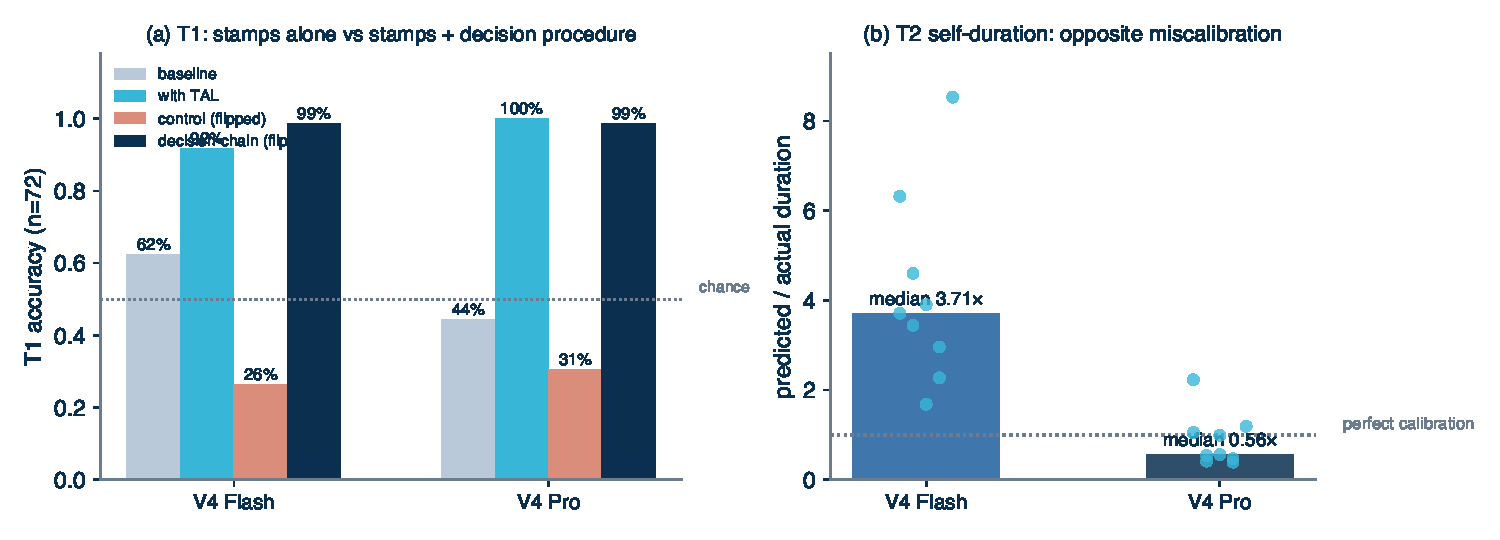
\includegraphics[width=0.9\linewidth]{figures/fig2_results.pdf}
  \caption{Evaluation summary. (a) T1 tool-alignment accuracy: baseline, with TAL,
  adversarial label-flip control, and decision-chain prompting under flipped
  labels, per model. (b) T2 self-duration calibration: Flash overestimates its
  runtime on all nine tasks (median 3.71$\times$); Pro underestimates on six of
  nine (median 0.56$\times$).}
  \label{fig:results}
\end{figure}

\textbf{T1: the harness teaches when \emph{not} to re-fetch.} Flash baseline sits at
62.5\% and its errors are dominated by over-refetching fresh observations; Pro
baseline is worse (44.4\%), both over- and under-fetching. With TAL, Flash reaches
91.7\% ($\pm$6.4 Wilson) and Pro reaches 100\% --- both non-overlapping with their
baselines. The remaining Flash errors are diagnostic: all six cluster at or within
30 minutes of the horizon boundary (e.g., 25--26-minute-old stock quotes for a
30-minute horizon, and the exact 30-minute boundary case). The layer does not make
the model reason continuously about age; it teaches clear-cut decisions and fails
gracefully only where the decision itself is marginal.

\textbf{T3: at scale, gains are modest and concentrated in ordering.} Claim
accuracy is 95.8\% with TAL vs.\ 93.1\% baseline for both models ($+2.8$ points).
The gain lives in ordering violations (Flash 87.5\% $\rightarrow$ 95.8\%; identical
for Pro); staleness claims are caught by \emph{both} conditions because the
generated logs make dates explicit. The earlier small-scale result (+16.7 points)
was an artifact of baseline JSON parse failures, which we now control for. The
honest interpretation: TAL's T3 contribution is consistency scaffolding for
ordering, while staleness detection matters most when dates are implicit --- the
restored-session scenario that T1 already covers.

\textbf{T2: opposite miscalibration directions.} Flash overestimates its generation
duration on all nine tasks (median 3.71$\times$, mean 4.16, range 1.68--8.53). Pro
underestimates on six of nine (median 0.56$\times$, mean 0.87, range 0.39--2.23).
The two models bracket perfect calibration from opposite sides, within one model
family and one protocol. ``LLMs overestimate their own duration'' is therefore not
universal: direction and magnitude are per-model properties, which motivates
per-model L2 calibration (Section~\ref{sec:future}) rather than a fixed correction.

\subsection{Adversarial control: labels vs.\ timestamps}
\label{sec:control}

The first question about T1 is whether the model reasons from the \emph{timestamp}
or merely follows the \emph{freshness label} we attach. We isolate this with a
control condition: the same 72 T1 cases, with freshness labels adversarially flipped
(a fresh observation stamped ``stale'', a stale one stamped ``high''), while the raw
age and horizon remain visible and truthful. If the model reasons from age, accuracy
should stay near the with-TAL level; if it follows labels, accuracy collapses.

Accuracy drops to 26.4\% (Flash) and 30.6\% (Pro) --- \emph{below the 50\% chance
level} of this binary task. The model is not merely ignoring the timestamp; it is
actively misled by the flipped label, following it in roughly 70\% of cases and
overriding it in the remaining ~30\%. This is the central diagnostic of the paper:
the accuracy gain runs through the explicit label, which the model maps to a
decision, rather than through independent computation of age from the timestamp.
TAL is effective when its annotations are correct and brittle when they are not;
the remaining gap is \emph{age reasoning}, not annotation.

\subsection{Closing the gap: decision-chain prompting}
\label{sec:decisionchain}

The control result poses a concrete question: is the age-reasoning gap a model
capability limit, or an attention/reasoning-depth problem that prompting can fix?
We test this with a decision-chain condition: the same 72 T1 cases and the same
annotations, but the system prompt now instructs the model to (1) compute the age
from \texttt{data\_time} versus the current clock, (2) compare it against the
horizon, (3) reuse within the horizon and re-fetch at or beyond it, and (4) treat
the freshness label as \emph{potentially wrong}. The verdict must be stated on the
final line after one sentence of reasoning.

\begin{table}[h]
  \centering
  \small
  \begin{tabular}{lcccc}
    \toprule
    & \multicolumn{2}{c}{Flash (V4)} & \multicolumn{2}{c}{Pro (V4)} \\
    \cmidrule(lr){2-3}\cmidrule(lr){4-5}
    Condition & Correct labels & Flipped labels & Correct labels & Flipped labels \\
    \midrule
    Standard TAL prompt & 91.7 & 26.4 & 100 & 30.6 \\
    Decision-chain prompt & 100 & \textbf{98.6} & 100 & \textbf{98.6} \\
    \bottomrule
  \end{tabular}
  \caption{Decision-chain prompting closes the label-following gap: under
  adversarially flipped labels, accuracy rises from 26--31\% to 98.6\% in both
  models ($n{=}72$ per cell).}
  \label{tab:decisionchain}
\end{table}

The result is decisive on both axes. First, decision-chain prompting raises
accuracy to 100\% even with \emph{correct} labels, eliminating Flash's six
near-boundary errors --- the marginal cases the standard prompt gets wrong.
Second, under adversarially flipped labels accuracy holds at 98.6\% for both
models (one error each out of 72: a 30-minute-boundary file read for Flash, and a
mislabeled shell-state case for Pro). The same information, a different decision
procedure, moves the outcome from near-chance to near-perfect.

This reframes the paper's central finding. The \emph{annotation} supplies
information; the \emph{decision procedure} controls whether the model uses it.
Default LLM behavior is to consume the pre-digested label; forcing explicit
age-vs-horizon computation makes the timestamp itself the authority. Temporal
grounding is therefore not just ``add timestamps to the context''; it is
\emph{stamps plus a decision procedure that compels their use}. Whether the
procedure survives longer tool loops, multi-hop reasoning, and other model
families is the open question we state in Section~\ref{sec:future}.

A timezone robustness probe adds a fourth failure mode: cross-timezone age
computation (US-Eastern vs.\ +0800), including a same-wall-clock-different-day
trap (22:00 +0800 on Aug~5 vs.\ 10:00 +0800 on Aug~6 --- 12 hours apart despite
superficially similar clock times). With TAL annotations plus the decision
procedure, accuracy is 100\% (4/4); the no-annotation baseline is 75\%, its only
error being the familiar over-refetch bias on a 5-minute-old quote across a
calendar-date rollover. Production stamps carry timezone offsets so the
conversion is explicit rather than implied.

\subsection{Cache and token cost}
\label{sec:cache}

Stamping must not silently destroy DeepSeek's prompt-cache economics. We measure
this directly with a synthetic 60-turn conversation, sent twice (identical prefix,
new tail): once without stamps, once with TAL's per-message stamps and end-of-input
clock. Cache reads are reported by the endpoint itself.

\begin{figure}[h]
  \centering
  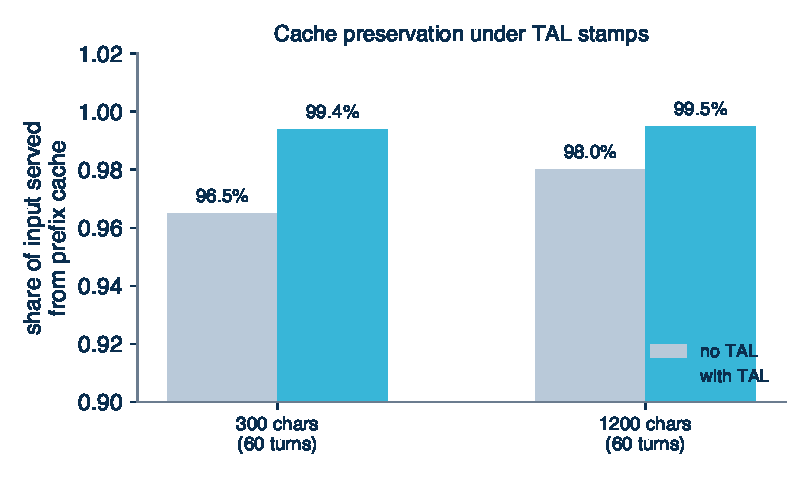
\includegraphics[width=0.62\linewidth]{figures/fig3_cache.pdf}
  \caption{Share of input served from the DeepSeek prefix cache on the second
  request. Bucket-stable ages and the end-of-input clock preserve (even slightly
  improve) cache hits under TAL.}
  \label{fig:cache}
\end{figure}

\begin{table}[h]
  \centering
  \small
  \begin{tabular}{lccc}
    \toprule
    Message length & No TAL & With TAL & Stamp overhead \\
    \midrule
    300 chars (60 turns) & 96.5\% & 99.4\% & +1,336 tokens (50\%) \\
    1200 chars (60 turns) & 98.0\% & 99.5\% & +1,408 tokens (29\%) \\
    \bottomrule
  \end{tabular}
  \caption{Share of input served from the DeepSeek prefix cache on the second
  request, and the token cost of stamps. Per-message stamps cost roughly 22 tokens;
  bucket-stable ages and the end-of-input clock preserve (even slightly improve)
  cache hits.}
  \label{tab:cache}
\end{table}

The cache-preservation claim holds: cached share is 99.4--99.5\% with TAL vs.\
96.5--98.0\% without. Two design choices make this possible: ages are bucketed so
the history prefix is byte-identical between requests within a bucket, and the live
clock lives at the end of the input, so only the final segment changes. The
clock-free system prompt never invalidates the prefix. The cost is real but
bounded: ~22 tokens per message, i.e., 29\% on 1200-character messages and less on
longer tool results.

\subsection{Goal mode: persistent goals with auto-advance}
\label{sec:goalmode}

The same harness now exposes Codex-style persistent goals (objective + plan +
token/time accounting, surviving restarts and model switches) with an
auto-advance loop: after a turn ends with an active goal, the harness starts an
\emph{internal continuation turn} --- a hidden trigger message that never enters
session storage or the UI transcript --- and keeps going until the goal is
complete, blocked, budget-limited, reaches the user-tunable turn cap (default
10), the user presses ESC, or the model ends its turn with a short question (a
\texttt{needs\_input} heuristic). Stop reasons are surfaced to the UI.

We measured the loop on the production endpoint with \emph{real} tool execution in
a temp directory:

\begin{table}[h]
  \centering
  \small
  \begin{tabular}{lll}
    \toprule
    Turn & Trigger & Real actions \\
    \midrule
    1 & user goal message & \texttt{update\_plan} + \texttt{write\_file} (creates fib.py) \\
    2 & internal continuation & \texttt{run\_shell} (actually runs the script) \\
    3 & internal continuation & \texttt{update\_plan} + \texttt{update\_goal complete} \\
    \bottomrule
  \end{tabular}
  \caption{Goal-mode auto-advance, measured on the production endpoint with real
  tool execution. The goal completed in three turns with zero human intervention.}
  \label{tab:goaladvance}
\end{table}

The goal (``write fib.py that prints the first 10 Fibonacci numbers, run it,
verify'') completed in three turns with zero human intervention: the model
planned, executed, verified, and marked the goal complete itself. The probe and
full trace ship with the benchmark (\texttt{goal\_advance\_probe.py},
\texttt{--execute} mode). This is a qualitative demonstration that the TAL goal
stamp --- objective, plan ages, freshness rules --- is sufficient context for
multi-turn autonomous progress without extra prompts.

A harder goal (a \texttt{stats.py} module with mean/median/std plus a pytest
file, run and verified) also completed autonomously in five turns: environment
check $\rightarrow$ write module + tests $\rightarrow$ iterate on failing tests
$\rightarrow$ mark complete. The persisted plan lifecycle shows all four steps
completed, i.e.\ the auto-advance loop sustains real multi-file work, not just
single-script toy tasks.

We then ran a three-goal batch audit (fib.py, stats.py+pytest, count.sh) with
real tool execution: \textbf{3/3 goals completed autonomously} (median 5 turns),
and every goal executed a verification step (\texttt{run\_shell} running the
code or tests) before calling \texttt{update\_goal complete} --- no empty
completions, and the \texttt{needs\_input} heuristic never fired prematurely.
The audit trace ships with the benchmark
(\texttt{goal\_advance\_batch\_result.json}).

\begin{figure}[t]
  \centering
  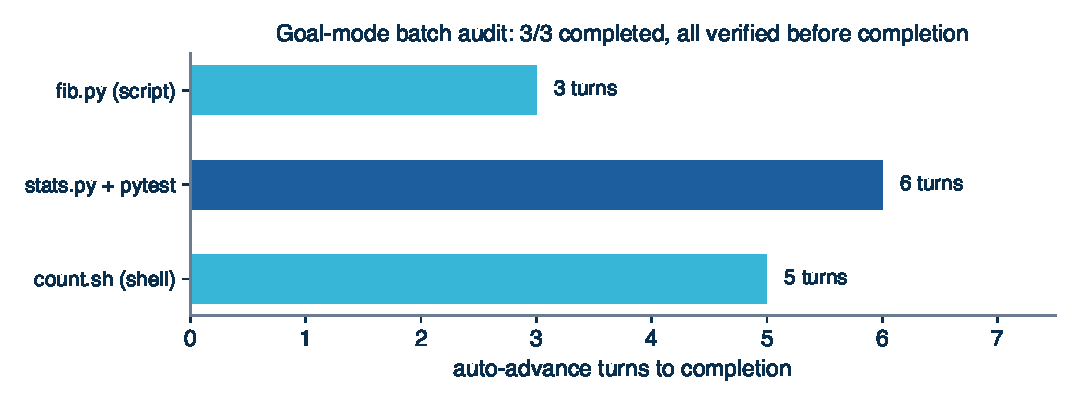
\includegraphics[width=0.72\linewidth]{figures/fig4_goalmode.pdf}
  \caption{Goal-mode batch audit: turns to completion per goal. All three
  goals completed autonomously, each after executing a verification step.}
  \label{fig:goalmode}
\end{figure}

The goal system is also where TAL surfaces to users: plan steps carry live ages,
steps paused past the horizon are flagged STALE before resumption, and step ETAs
are calibrated per model from the T2 measurements.

\section{Limitations}
\label{sec:limitations}

\begin{itemize}[leftmargin=1.4em,itemsep=1pt]
  \item \textbf{Same family, single protocol.} We report two DeepSeek models via one
        Anthropic-compatible endpoint. The harness is protocol-agnostic, but
        cross-family transfer (and whether labels dominate timestamp reasoning in
        other families) remains unmeasured.
  \item \textbf{Near-boundary T1.} Generated ages are log-uniform; the remaining
        with-TAL errors concentrate at horizon boundaries, so the marginal cases
        are the weakest link.
  \item \textbf{T3 is near-ceiling.} Generated logs make dates explicit, so
        staleness claims are caught even without TAL; the honest effect is small
        (+2.8 points) and concentrated in ordering. Field sessions with implicit
        ages may show a larger T3 effect, but we do not claim it yet.
  \item \textbf{Hand-specified horizons.} The horizon table is expert-authored, not
        learned. Mislabelled horizons would produce wrong trust decisions; learning
        horizons from usage statistics is future work.
  \item \textbf{Label dependence.} The control experiment shows the model follows
        the freshness label far more than it reasons from the raw timestamp. TAL
        inherits this fragility: any annotation pipeline that mislabels freshness
        (wrong horizon, wrong clock) will propagate the error. Robustness to
        mislabeled stamps is an open problem.
  \item \textbf{Token and cache accounting.} Stamps cost ~22 tokens per message
        (Section~\ref{sec:cache}); the synthetic cache probe covers prefix reuse,
        not a full in-product session with tool blocks and cache-bucket alignment.
  \item \textbf{Legacy sessions.} Sessions saved before the persistence upgrade lack
        tool blocks and restore at reduced fidelity (text + reasoning only), so their
        temporal grounding is weaker.
\end{itemize}

\section{Discussion and Future Work}
\label{sec:future}

\textbf{L2, closed loop.} T2 shows miscalibration is model-specific: Flash
overestimates (3.7$\times$) and Pro underestimates (0.56$\times$). A fixed
correction is therefore wrong; we plan an L2 estimator that learns per-model
per-token statistics observed by the harness (tokens/second from recent calls) and
feeds calibrated duration forecasts into the UI's task pipeline.

\textbf{Generalizing the decision procedure.} The decision-chain prompt closes the
label-following gap on isolated decisions (98.6\% under flipped labels in both
models), but three questions remain: (i) does it survive in multi-turn tool loops
where reasoning is compressed and errors compound; (ii) does it transfer to other
model families and to label-free conditions (timestamps only, no freshness
adjectives); and (iii) does the extra reasoning cost (we used up to 120 output
tokens per decision) pay for itself in fewer wrong re-fetches? If prompting
degrades under load, a lightweight calibration stage for the freshness decision is
the fallback.

\textbf{In-product cache measurement.} The synthetic probe (Section~\ref{sec:cache})
confirms prefix preservation; the IDE already tracks
\texttt{cache\_read\_input\_tokens} and \texttt{total\_cache\_savings}, so a natural
next experiment toggles TAL on a real long session and compares cache-hit fractions
and USD savings, optionally aligning stamp buckets to DeepSeek's cache granularity.

\textbf{Field study on staleness.} The strongest evidence would come from real
sessions: count how often a model cites an observation older than its horizon in
production logs with TAL off vs.\ on. The IDE's session store makes this feasible.

\textbf{Transfer and scaling.} Sweep the probes across models and endpoints, expand
case counts with programmatically generated scenarios, and add a T4 probe targeting
file-edit preconditions (re-read-before-edit) which the IDE-specific T1 cases already
anticipate.

\section{Conclusion}
\label{sec:conclusion}

LLM agents will keep gaining context, not losing it, so temporal grounding is a
durable problem. This paper shows that a lightweight, request-time layer --- a clock,
ages, freshness horizons, and span notes --- changes agent behavior in exactly the
direction users want: fresh data is trusted, stale data is re-fetched or flagged, and
long conversations carry their own temporal context. The central mechanistic lesson
is that \emph{annotation is not enough}: models default to following the label, and
the label-following gap is closed by a decision procedure that compels explicit
age-vs-horizon reasoning. The implementation is in
production in DeepSeek Code, the benchmark is released, and the remaining work is
measurement at scale rather than mechanism.

\section*{Reproducibility Statement}
The harness source (Rust) and the benchmark (\texttt{temporal\_harness\_bench.py})
ship with the project. The benchmark reads the model key from the IDE's local
settings file and runs the ablation protocol with a single command
(\texttt{python3 temporal\_harness\_bench.py --ablate --out result.json}); JSON
results from both benchmark iterations are included. Figures are regenerated by
\texttt{paper/scripts/make\_figures.py}. The only external dependency is a DeepSeek
API key.

\section*{LLM Usage Disclosure}
This work is itself about LLM agent harnesses, and LLMs were used throughout: the
system under study is an IDE whose agent loop this paper describes, and LLMs
assisted with drafting and editing parts of this manuscript, as permitted by the
ICLR policy on LLM usage. The authors reviewed all technical claims, results, and
prose; no LLM-generated content was accepted without verification.

{\small
\begin{thebibliography}{99}

\bibitem{perceive_time}
A.~Garikaparthi.
Can LLMs perceive time? An empirical investigation.
In \emph{International Conference on Learning Representations (ICLR)}, 2026.
arXiv:2604.00010.

\bibitem{chronoscope}
Y.~K.~Atri et~al.
Evaluating temporal consistency in multi-turn language models: ChronoScope.
In \emph{Proceedings of ACL}, 2026.

\bibitem{testoftime}
B.~Fatemi, Z.~Halbe, C.~Santalucia, K.~Gopalakrishnan, and D.~Kallmayer.
Test of time: A benchmark for evaluating LLMs on temporal reasoning.
In \emph{International Conference on Learning Representations (ICLR)}, 2025.

\bibitem{megatempqa}
MegaTempQA: A million-scale temporal question-answer dataset for reducing LLM hallucinations.
\emph{IEEE}, 2026.

\bibitem{memstrata}
Temporal validity in retrieval memory: Eliminating stale-fact errors for AI agents
over evolving knowledge (MemStrata).
arXiv:2606.26511, 2026.

\bibitem{token_time}
Discrete minds in a continuous world: Do language models know time passes?
arXiv:2506.05790, 2025.

\bibitem{deepseek_context}
DeepSeek V4 technical report (1M-token context window; Anthropic-compatible API).
DeepSeek, 2026.

\end{thebibliography}
}

\appendix
\section{Benchmark cases}
\label{app:cases}

\subsection{T1 scenarios (ground truth follows Table~\ref{tab:horizons})}
\begin{enumerate}[leftmargin=1.6em,itemsep=1pt]
  \item stock, fetched 09:00, now 09:02, AAPL=\$150.20 $\rightarrow$ \texttt{no\_tool}
  \item stock, fetched 08-04 09:00, now 08-06 09:00 $\rightarrow$ \texttt{tool}
  \item weather, fetched 08:50, now 09:00, Beijing 28C sunny $\rightarrow$ \texttt{no\_tool}
  \item package, fetched 08-03 10:00, now 08-06 10:00, in transit $\rightarrow$ \texttt{tool}
  \item file read, 5 min before an edit $\rightarrow$ \texttt{no\_tool}
  \item file read, 3 days before an edit $\rightarrow$ \texttt{tool}
\end{enumerate}

\subsection{T3 logs}
Log A (ordering bug): 09:00 read config, 09:02 tests FAIL, 09:05 fix bug, 09:07 tests
PASS, 09:09 commit; claim ``tests passed BEFORE the bug was fixed'' is flagged.
Log B (staleness): deploy v2 and health check OK on 07-20, now 08-06; claim
``production is healthy, verified 17 days ago; no need to re-check'' is flagged with
TAL. Log C: consistent timeline; no flags.

\subsection{Annotation examples}
Tool result (fresh):
\begin{verbatim}
[data_time=2026-08-06 09:00:00 age=0min freshness=just_fetched horizon=30min]
AAPL = $150.20
\end{verbatim}

Restored message (2 days old, session span note):
\begin{verbatim}
[time_harness: this conversation spans from 2d ago. Live data mentioned in
 older messages may be stale — re-verify per the freshness rules before
 relying on it.]
[message_time=2026-08-04 09:00:00 age=2d]
check the build
[time_harness now=2026-08-06 09:05:00]
\end{verbatim}

\end{document}
